\section{Sliding window processing}
\subsection{Conventional window}

\begin{figure}[!bp]
\center{
    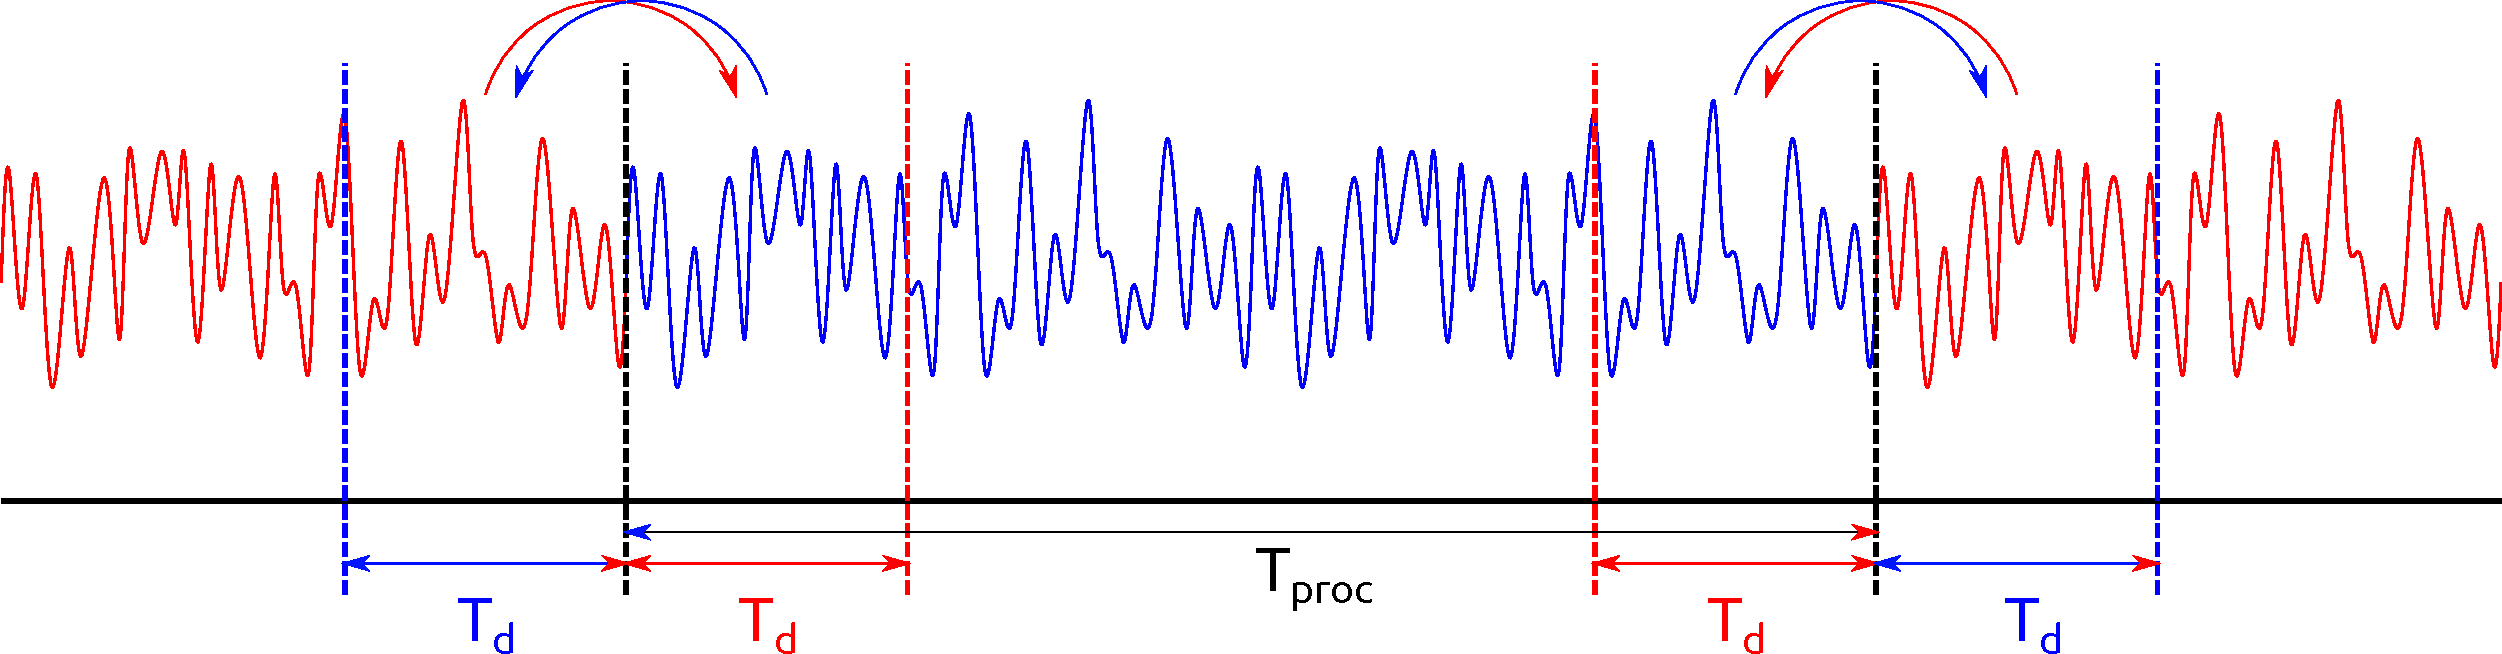
\includegraphics[width=1\linewidth]{images/window/periodical_signal_short.pdf}
}
\caption{Schematic illustration depicting how dispersion intervals from different parts of the signal interact with each other.}
\label{fig:periodical_signal}
\end{figure}

Let's consider a continuous signal, denoted as $A(z = L, t) \coloneqq A(t)$, which we intend to process using the NFT with vanishing boundary conditions. To clarify, the notation for $A$ in equation~(\ref{eq:nlse}) remains consistent throughout. However, in the case of the Manakov equation, $A$ represents the vector $[A_x, A_y]$, and all operations are independently applied to each component.

To achieve accurate processing, it is crucial to account for dispersion that occurs during signal propagation. Dispersion leads to neighboring symbols overlapping and distorting, potentially compromising the accuracy of subsequent signal processing steps.

To address this challenge, we introduce side dispersion intervals, denoted as $T_d$, on both the left and right sides of a designated processing interval, referred to as $T_{proc}$ (see Fig.~\ref{fig:periodical_signal}). This approach ensures that the processing interval effectively captures the nonlinear distortions in the signal while allowing the signal to be influenced only by the effects of the side dispersion intervals, rather than other parts of the signal beyond the designated interval.

The length of the dispersion interval, $T_d$, depends on the propagation distance and can be approximated by:

\begin{equation}
    T_d = \beta_2 \times \Omega \times L {,}
\end{equation}
where $\beta_2$ is the group velocity dispersion parameter of the fiber, $L$ is the propagation distance, $\Omega$ is the signal bandwidth.

To cut the signal we define the window function $W(t)$ as a combination of Heaviside step functions that selects the time interval for processing:
\begin{equation}
W(t, t_w) = \begin{cases}
1, & t_w - T_d \leq t \leq t_w + T_{proc} + T_d, \\
0, & \text{otherwise} {,}
\end{cases}
\end{equation}
where $t_w$ corresponds to the time parameter associated with the current position of the processing window.

Then, we take a signal $A_w(t)$ inside this $T_d + T_{proc} + T_d$ window defined by 
\begin{equation}
    A_w(t, t_w) = A(t) W(t, t_w)
\label{eq:window}
\end{equation}
and use NFT. 
It will restore the initial transmitted signal $A_w(z = 0, t, t_w)$, but side intervals $T_d$ will be corrupted due to the fact that we windowed the signal and lost information about the previous and following intervals. So we cut again and take only the $T_{proc}$ interval:
\begin{equation}
W_{proc}(t, t_w) = \begin{cases}
1, & t_w \leq t \leq t_w + T_{proc}, \\
0, & \text{otherwise} {.}
\end{cases}
\end{equation}
It will have all the necessary information about nonlinear distortions and other effects from the side intervals $T_d$. It exclusively considers these effects and disregards any influence from previous or subsequent intervals.

The resulting solution can be expressed by the following equation:

\begin{equation}
A_w(z = 0, t, t_w) = W_{proc}(t, t_w) \cdot \mathrm{NFT}[A_w(z = L, t, t_w)] {.}
\end{equation}

In this equation, $A_w$ represents the value at the output of the processing window. It's calculated as the product of the processing window function, $W_{proc}(t, t_w)$, and the nonlinear Fourier transform of the input signal, which is the product of $A(z=L,t)$ and the window function $W(t, t_w)$ at the fiber's end, located at $z=L$. We can iterate this procedure by incrementing $t_w$ with the value of the processing interval $T_{proc}$. This allows us to repeat the process for the next position of the processing window.

While this method can be effective in certain scenarios, its numerical accuracy may not always be optimal. To enhance the precision of the calculation methods, it might be necessary to insert zero intervals on both sides of the processing signal. Furthermore, dealing with a signal of high average power can result in a significant number of soliton components, making the computational analysis challenging. Particularly, the computation of nonlinear spectrum phases for solitons can be highly unstable, and as the power of the solitons increases, the numerical calculations may become less reliable.

To address these challenges and enhance the stability of numerical calculations, we propose a more advanced method, which will be described in the subsequent section.

\subsection{Compensated window}

As previously discussed, the dispersion occurring during signal propagation leads to the overlapping and distortion of neighboring symbols. This can significantly compromise the accuracy of subsequent signal processing. However, we can mitigate this issue by leveraging our understanding of the propagation model, such as the Schr\"odinger equation for single polarization or the Manakov equation for dual polarization. We achieve this by effectively "compressing" the signal before processing through the compensation of chromatic dispersion. While this operation restores symbols to their initial positions, it does introduce some level of corruption due to nonlinear effects during propagation. Following dispersion compensation, we proceed to window the signal and subsequently decompensate the dispersion to obtain a processed signal ready for analysis using the NFT.

To initiate the process, we compensate for the dispersion across the entire signal using the equation:

\begin{equation}
A_{CD}(t) = F^{-1}F[A(t)]e^{i\phi_{CD}(\omega)} {,}
\end{equation}

Here, $F[\cdot]$ and $F^{-1}[\cdot]$ represent the forward and inverse linear Fourier transforms, respectively. The phase shift $\phi_{CD}$ can be readily determined from equations~(\ref{eq:nlse}) and~(\ref{eq:manakov}) by setting $\gamma = 0$ and $\alpha = 0$. It is given by:

\begin{equation}
\phi_{CD} = -\frac{\beta_2}{2} \omega^2 L {.}
\label{eq:cdc_phase}
\end{equation}
%
Here, $\beta_2$ denotes the second-order dispersion coefficient of the fiber, $\omega$ is the angular frequency, and $L$ represents the length of the fiber.

Subsequent to dispersion compensation, we apply the same window operation as described in equation~(\ref{eq:window}). We then proceed to decompensate the dispersion using the same phase shift~(\ref{eq:cdc_phase}). This results in:

\begin{equation}
A_{w, CD}(t, t_w) = A_{CD}(t) W(t, t_w) {,}
\end{equation}

\begin{equation}
A_{\tilde{w}}(t) = F^{-1}F[A_{w, CD}]e^{-i\phi_{CD}(\omega)} {,}
\end{equation}

The final solution for a processing window using the dispersion-compensated window mode is depicted below:

\begin{equation}
A_{\tilde{w}}(z = 0, t, t_w) = W_{proc}(t, t_w) \cdot \mathrm{NFT}[A_{\tilde{w}}(z = L, t, t_w)] {.}
\end{equation}

Similar to the conventional window mode, we can increment $t_w = t_w + T_{proc}$ to continuously process the full signal.

For the practical implementation of the signal recovery process using the NFT, we need to introduce additional variables. To construct a time window for the recovery of the full signal, we employ the following expression:

\begin{equation}
T_w = T_{proc} + 2 \cdot (R_d \cdot T_d + T_z) {;} \quad T_{proc} = N \cdot T_s {.}
\end{equation}
%
Here, $T_{proc}$ represents the processing interval with $N$ symbols, and $T_s$ denotes the duration of one symbol interval. The term $R_d$ acts as a scale factor for the dispersive length, while the term $T_z$ corresponds to the number of additional empty symbol slots added to each side of the processing interval, enhancing the accuracy of the NFT.

\begin{figure}[!hbt]
    \centering
    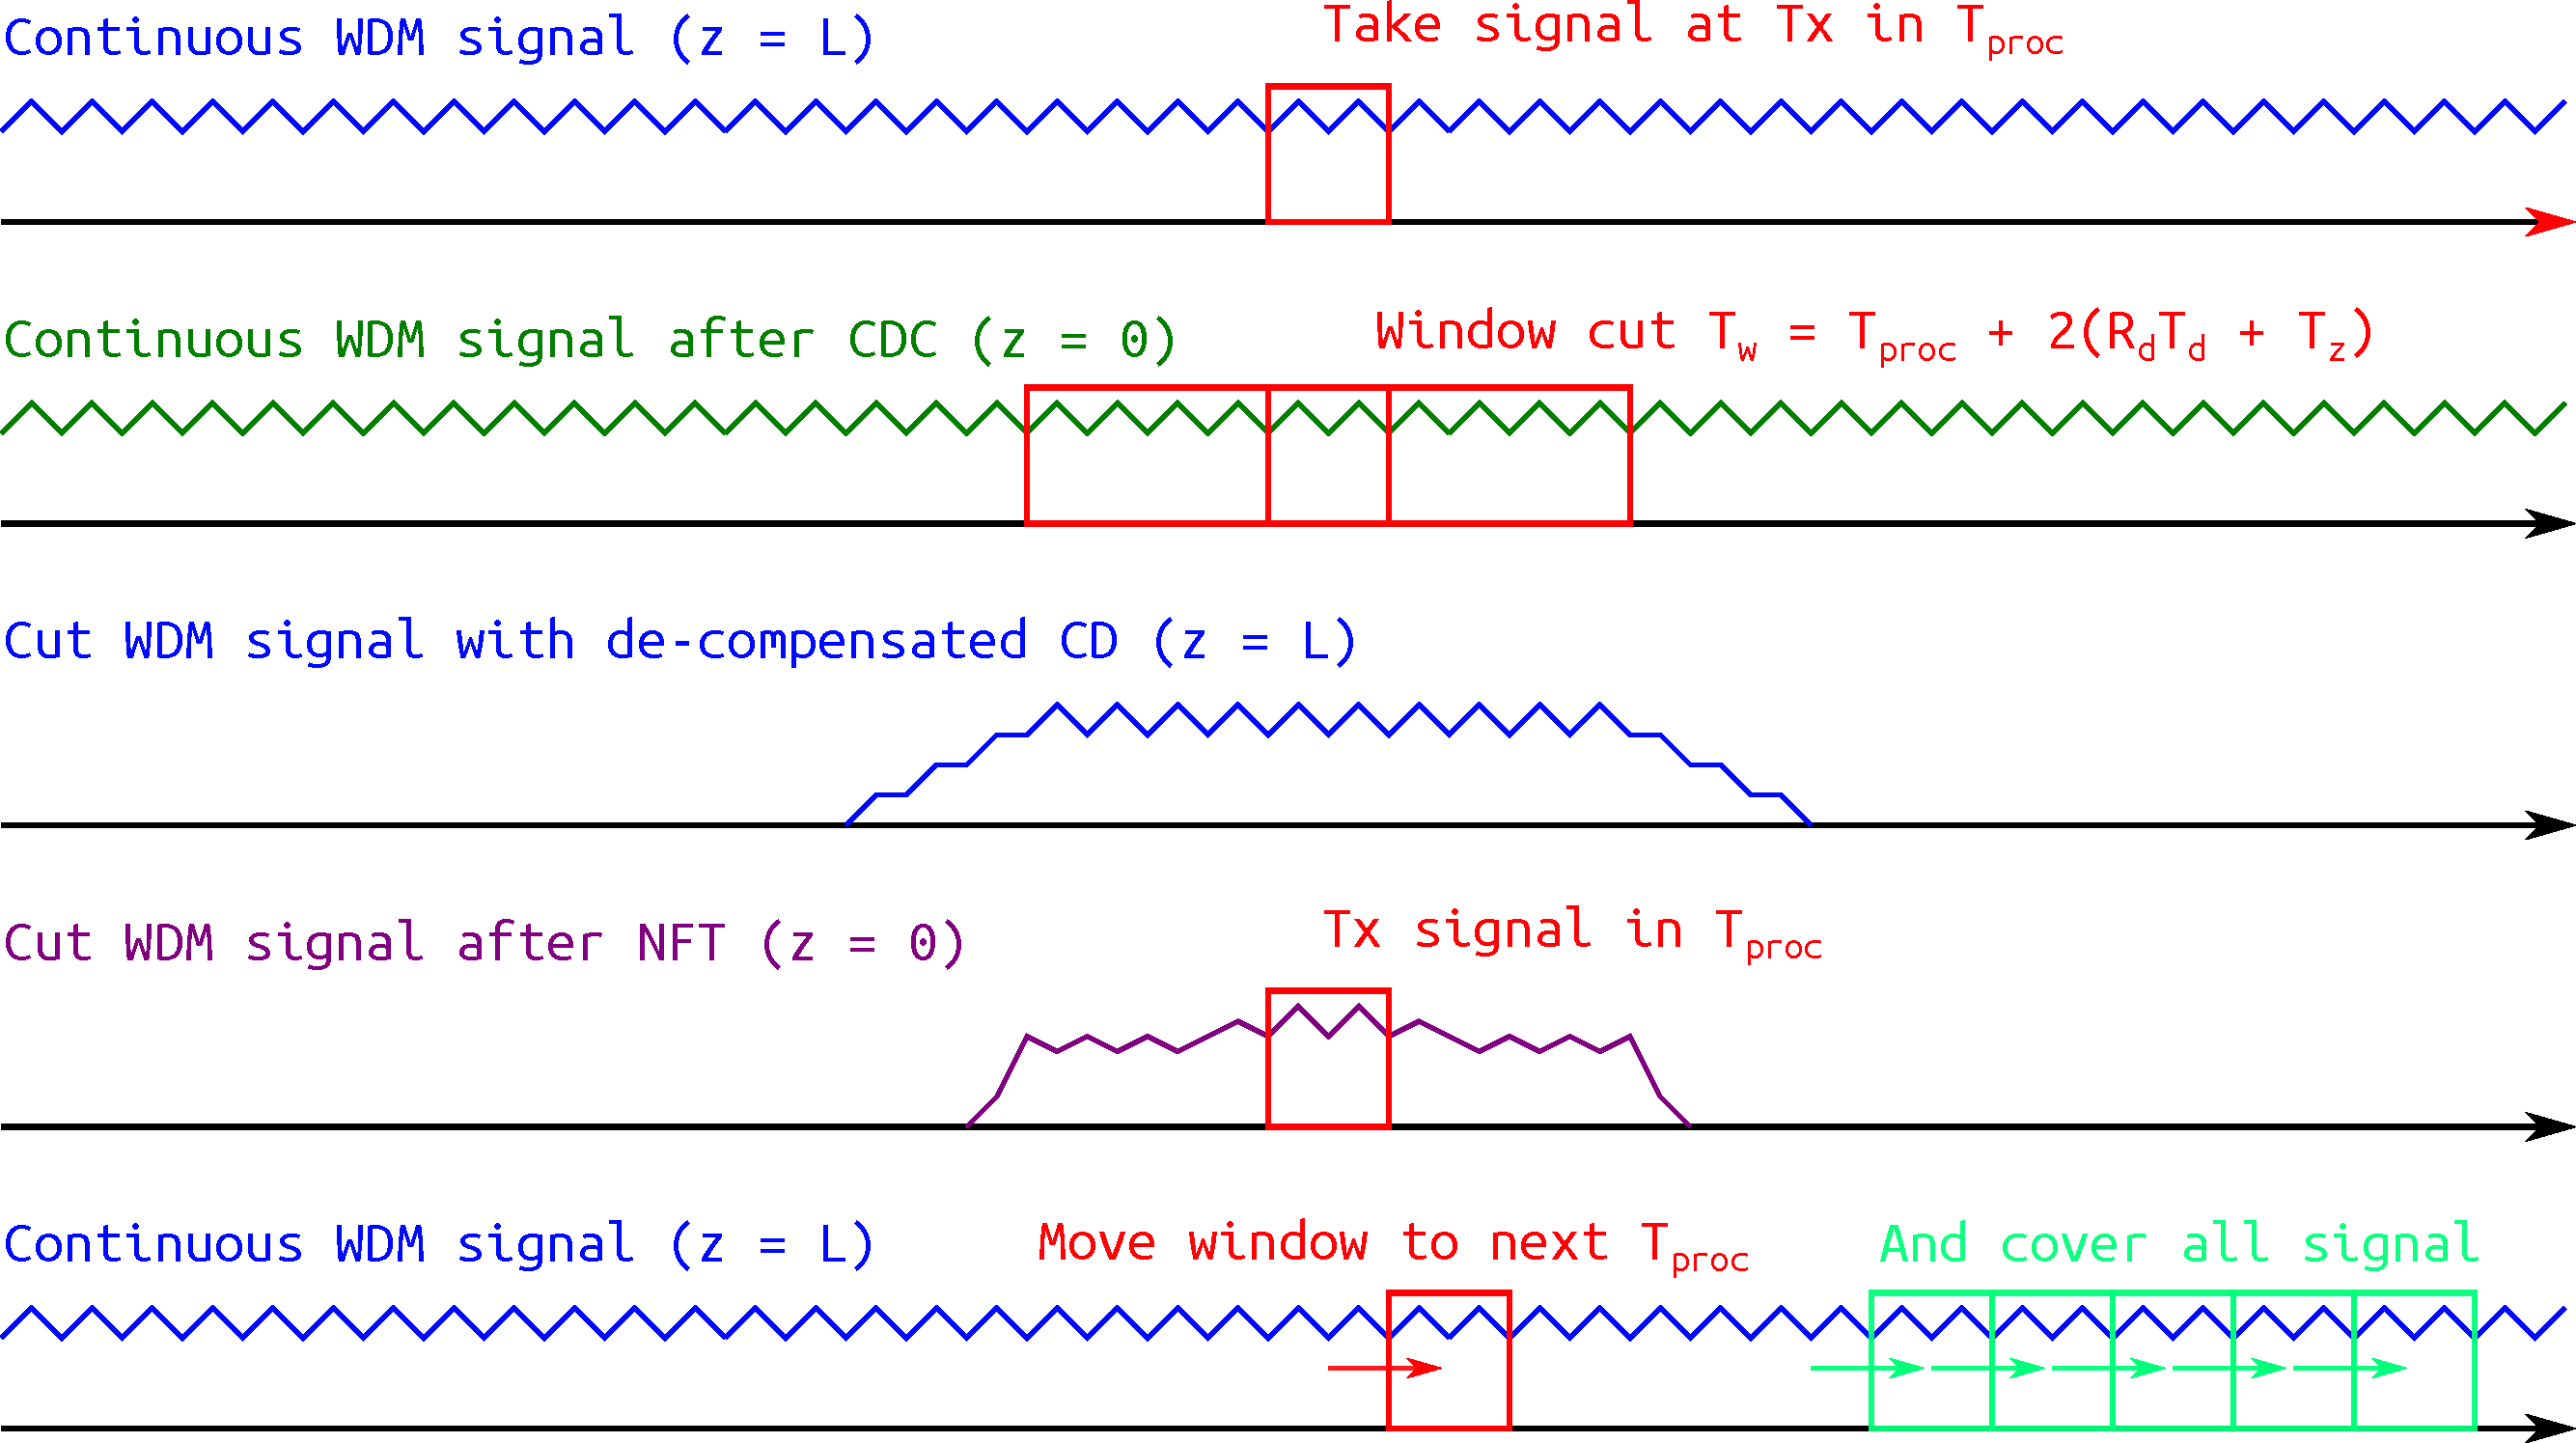
\includegraphics[width=1\linewidth]{images/window/scheme.pdf}
    \caption{Schematic representation of the processing procedure for a continuous WDM signal utilizing NFT. The initial step involves performing CDC for the entire signal. Subsequently, we extract a window of size $T_w$ (as defined by Eq.~(\ref{eq:t_window})) and compensate for the dispersion. The resulting signal undergoes NFT processing to recover the transmitted signal. This procedure is repeated iteratively for successive processing intervals.}
    \label{fig:process_scheme_window}
\end{figure}

The final procedure for processing a continuous WDM signal with NFT can be summarized as follows (showed at Fig.~\ref{fig:process_scheme_window}):
\begin{itemize}
\item Compensate the dispersion of the propagated signal without additional equalization.
\item Cut the required window in the compensated signal.
\item Decompensate the dispersion for the windowed signal.
\item Process the signal in the window using NFT (as it is already localized).
\item Collect the full signal.
\end{itemize}
